%
% The first command in your LaTeX source must be the \documentclass command.
\documentclass[sigconf]{acmart}
\definecolor{pblue}{rgb}{0.13,0.13,1}
\definecolor{pgreen}{rgb}{0,0.5,0}
\definecolor{pred}{rgb}{0.9,0,0}
\definecolor{pgrey}{rgb}{0.46,0.45,0.48}
\usepackage{tabularx}
\usepackage{listings}

\lstset{language=Java,
  showspaces=false,
  showtabs=false,
  breaklines=true,
  showstringspaces=false,
  breakatwhitespace=true,
  commentstyle=\color{pgreen},
  keywordstyle=\color{pblue},
  stringstyle=\color{pred},
  basicstyle=\ttfamily,
  moredelim=[il][\textcolor{pgrey}]{$$},
  moredelim=[is][\textcolor{pgrey}]{\%\%}{\%\%}
}

\def\code#1{\texttt{#1}}
\long\def\red#1{\textcolor{red}{#1}}

%
% defining the \BibTeX command - from Oren Patashnik's original BibTeX documentation.
\def\BibTeX{{\rm B\kern-.05em{\sc i\kern-.025em b}\kern-.08emT\kern-.1667em\lower.7ex\hbox{E}\kern-.125emX}}

% Rights management information.
% This information is sent to you when you complete the rights form.
% These commands have SAMPLE values in them; it is your responsibility as an author to replace
% the commands and values with those provided to you when you complete the rights form.
%
% These commands are for a PROCEEDINGS abstract or paper.
\copyrightyear{2019}
\acmYear{2019}
\setcopyright{acmlicensed}
\acmConference[LA-WEB 2019]{LA-WEB 2019: 10th Latin American Web Congress}{May 13-14, 2019}{San Francisco, CA, USA}
\acmBooktitle{LA-WEB 2019: 10th Latin American Web Congress. May 13-14, 2019. San Francisco, CA, USA}
% \acmPrice{15.00}
% \acmDOI{10.1145/1122445.1122456}
% \acmISBN{978-1-4503-9999-9/18/06}

%
% These commands are for a JOURNAL article.
%\setcopyright{acmcopyright}
%\acmJournal{TOG}
%\acmYear{2018}\acmVolume{37}\acmNumber{4}\acmArticle{111}\acmMonth{8}
%\acmDOI{10.1145/1122445.1122456}

%
% Submission ID.
% Use this when submitting an article to a sponsored event. You'll receive a unique submission ID from the organizers
% of the event, and this ID should be used as the parameter to this command.
%\acmSubmissionID{123-A56-BU3}

%
% The majority of ACM publications use numbered citations and references. If you are preparing content for an event
% sponsored by ACM SIGGRAPH, you must use the "author year" style of citations and references. Uncommenting
% the next command will enable that style.
%\citestyle{acmauthoryear}

%
% end of the preamble, start of the body of the document source.
\begin{document}

%
% The "title" command has an optional parameter, allowing the author to define a "short title" to be used in page headers.
\title[After Brazil's GDPR: Authorization in Decentralized Web Applications]{After Brazil's General Data Protection Law: Authorization in Decentralized Web Applications}

%
% The "author" command and its associated commands are used to define the authors and their affiliations.
% Of note is the shared affiliation of the first two authors, and the "authornote" and "authornotemark" commands
% used to denote shared contribution to the research.
\author{Jefferson O. Silva}
\email{silvajo@pucsp.br}
\affiliation{%
  \institution{Pontifical Catholic University of S\~ao Paulo}
  \city{S\~ao Paulo}
  \country{Brazil}
}

\author{Newton Calegari}
\email{newton@nic.br}
\affiliation{%
  \institution{Brazilian Network Information Center - NIC.br}
  \city{S\~ao Paulo}
  \country{Brazil}
}

\author{Eduardo S. Gomes}
\email{egomes@pucsp.br}
\affiliation{%
  \institution{Pontifical Catholic University of S\~ao Paulo}
  \city{S\~ao Paulo}
  \country{Brazil}
}

%
% By default, the full list of authors will be used in the page headers. Often, this list is too long, and will overlap
% other information printed in the page headers. This command allows the author to define a more concise list
% of authors' names for this purpose.
\renewcommand{\shortauthors}{Silva et al.}

%
% The abstract is a short summary of the work to be presented in the article.
\begin{abstract}
Currently, decentralized Web Applications (Web Apps) do not offer fine-grained access controls to users' data, which potentially creates openings for data breaches. For software companies that need to comply with Brazil's General Data Protection Law (LGPD), privacy violations could mean incurring in hefty fines. We propose the use of Esfinge Guardian framework for increasing compliance with the LGPD in the context of decentralized Web Apps.
\end{abstract}

%
% Keywords. The author(s) should pick words that accurately describe the work being
% presented. Separate the keywords with commas.
\keywords{Access Control, Decentralized Web Apps, Frameworks, Guardian, Solid}

%
% This command processes the author and affiliation and title information and builds
% the first part of the formatted document.
\maketitle

\section{Introduction}

With the approval of the Brazilian General Data Protection Law (LGPD, Portuguese acronym) \cite{LGPD18}, several software companies may need to redesign the applications that handle the personal data of Brazilian citizens. The LGPD considers personal any data that directly or indirectly lead to the identification of a user \cite{LGPD18}. Neglecting the LGPD requirements could mean incurring in fines up to 2\% of companies' global revenue \cite{LGPD18}.

The LGPD sets compliance requirements on the companies in charge of making decisions about the data processing (i.e., data controllers) and the companies that process personal data in the name of data controllers (i.e., data processors) \cite{LGPD18}. The LGPD states that, in some cases, data controllers and data processors may be held liable, especially in cases where data breaches are harmful to users \cite{LGPD18}.

To avoid being classified as either data processors or data controllers (as an attempt to avoid sanctions), some companies may redesign applications as decentralized Web Applications (Web Apps). In the context of this research, an application is considered decentralized when it does not hold users' data. Tim Berners-Lee and colleagues \cite{Sambra} propose a platform called Solid (derived from "\textbf{So}cial \textbf{li}nked \textbf{d}ata"), which can be described as a set of principles, conventions, and tools for building decentralized Web Apps. Solid is based on the principle that users should have full ownership of their data, which are stored in Web-accessible personal online datastores (pods) \cite{Sambra}. Pods are independent of Web Apps. For obtaining services, users need to authorize Web Apps to access their pods explicitly, by classifying Web Apps as trusted.

Using Solid alone leaves users solely responsible for controlling access to protected resources, which may not be enough to comply with the LGPD. The LGPD requirement of data governance (see Art. 50, Par. 2 in \cite{LGPD18}) states that, among other things, companies should establish adequate policies to protect users' data. Nevertheless, in Solid Web Apps, a user would not have the means to prevent unauthorized access to their data, after classifying a Web App as trusted. For example, a bank Web App may have a sensitive operation that reads personal data from the users' pods that should be accessible only by account managers. A violation of this access control policy would configure a data breach, in which case the bank might still be held liable. Also, the liability risk might create the need for audits, in which case it would be necessary that the company demonstrated that it possesses appropriate controls, possibly directly in source code.

Thus, we establish the following research question (RQ).

\vspace{0.15cm}
\noindent \textbf{RQ: How to design decentralized Web Apps to increase compliance with the LGPD requirement of data governance?}
\vspace{0.15cm}

We claim that the answer to our RQ may help companies to design authorization solutions in decentralized Web Apps in increased compliance with the LGPD.

This work is organized as follows. In Chapter 2, we offer some background. In Chapter 3, we present Esfinge Guardian. In Chapter 4, we offer a case example. In Chapter 5, we present some related works. We conclude with a brief discussion in Chapter 6.


\section{Background}
In this section, we offer some background on the Brazil's General Data Protection Law, on decentralized Web Apps in Solid, and on access control in Solid.

\subsection{Brazil's General Data Protection Law}

The Brazil's General Data Protection Law (LGPD) is based on the General Data Protection Regulation (GDPR),\footnote{\url{http://data.consilium.europa.eu/doc/document/ST-9565-2015-INIT/en/pdf}} which aims at protecting the personal data of EU individuals. In total, around 120 countries adopt comprehensive privacy laws and regulations to protect personal data held by private and public bodies \cite{Banisar2011}.

The LGPD applies to any individual or legal entity (public or private) with personal data processing activities that: are carried out in Brazil; offer or supply goods or services in Brazil or relate to individuals located in Brazil, and; involve personal data collected in Brazil.

The LGPD also requires companies to nominate a Data Protection Officer who will be in charge of monitoring the adoption of best practices for personal data protection and for reporting to the National Data Protection Authority.

\subsection{Decentralized Solid Web Apps}

Traditional Web Apps (e.g., Facebook, Twitter, and Santander) implement private APIs, access control and data storage mechanisms. Because users cannot move their data to other platforms, these Web Apps become "data silos." We refer to these Web Apps as centralized Web Apps.

Solid is a platform that supports decentralized Web Apps, by relying on open standards and semantic web technologies. In the Solid platform, applications run in a browser or as mobile applications, while users data are stored in a Web-accessible personal online data store (pods). However, protocols for access controls, communications between servers and applications are specific to Solid \cite{Sambra}.

Data used by Solid Web Apps are stored in users' pods. Although pods can be stored locally or remotely, they typically are stored in pod servers. Pod servers manage data according to the Linked Data Platform recommendation, enabling it to manipulate data items through HTTP requests \cite{LDP}. Solid servers are application-agnostic and can deal with both structured and unstructured data. Structured data is represented using RDF, a Semantic Web standard. Application development based on Solid platform supports portability and interoperability, so applications can be seen as an interface that works with distributed data in multiple pod server implementations.

Identity in the Solid context is based on WebID, which allows agents (a person, an organization, etc.) to create their identities using global unique identifiers - HTTP URIs \cite{Sambra}. A WebID is an open and decentralized identification mechanism being developed by a W3C community group.\footnote{\url{https://www.w3.org/community/webid/}}

The main idea behind Solid is to put people back in control of their data, allowing them to choose where to store their data. Solid aims at aligning with the view of a decentralized web, where data is decentralized and stored in personal data storages, or distributed servers in which the user has full control over its data \cite{verborgh_iswc_2018}.

In a decentralized web model, resources created using one application and can be read and modified by a different one without prior agreement between the applications. It is possible because the applications are interfaces to access data stored in multiple locations, such as in a pod.

\subsection{Access Control in Solid}

Access control is typically split into two distinct procedures: authentication, and authorization. While authentication is concerned with determining whether an agent (e.g., user, group) is whom it claims to be, authorization is responsible for verifying if the agent is allowed to access a protected resource (e.g., document) or operation (e.g., read, write, append).

The Solid project uses the Web Access Control (WAC) specification for controlling the access to protected resources. WAC specifies a decentralized cross-domain access control system, similar to existing access control models. According to the specification, WAC has the following key features:

\begin{enumerate}
\item The resources are identified by URLs and can refer to any web documents or resources.
\item It is declarative -- access control policies are written in regular web documents.
\item Users and groups are also identified by URLs (specifically, by WebIDs).
\item It is cross-domain -- all of its components, such as resources, agent WebIDs, and even the documents containing the access control policies, can potentially reside on separate domains.
\end{enumerate}


\begin{lstlisting}[escapeinside=||,caption={Example WAC Document}, captionpos=b,label={lst:individual-permission}]
  |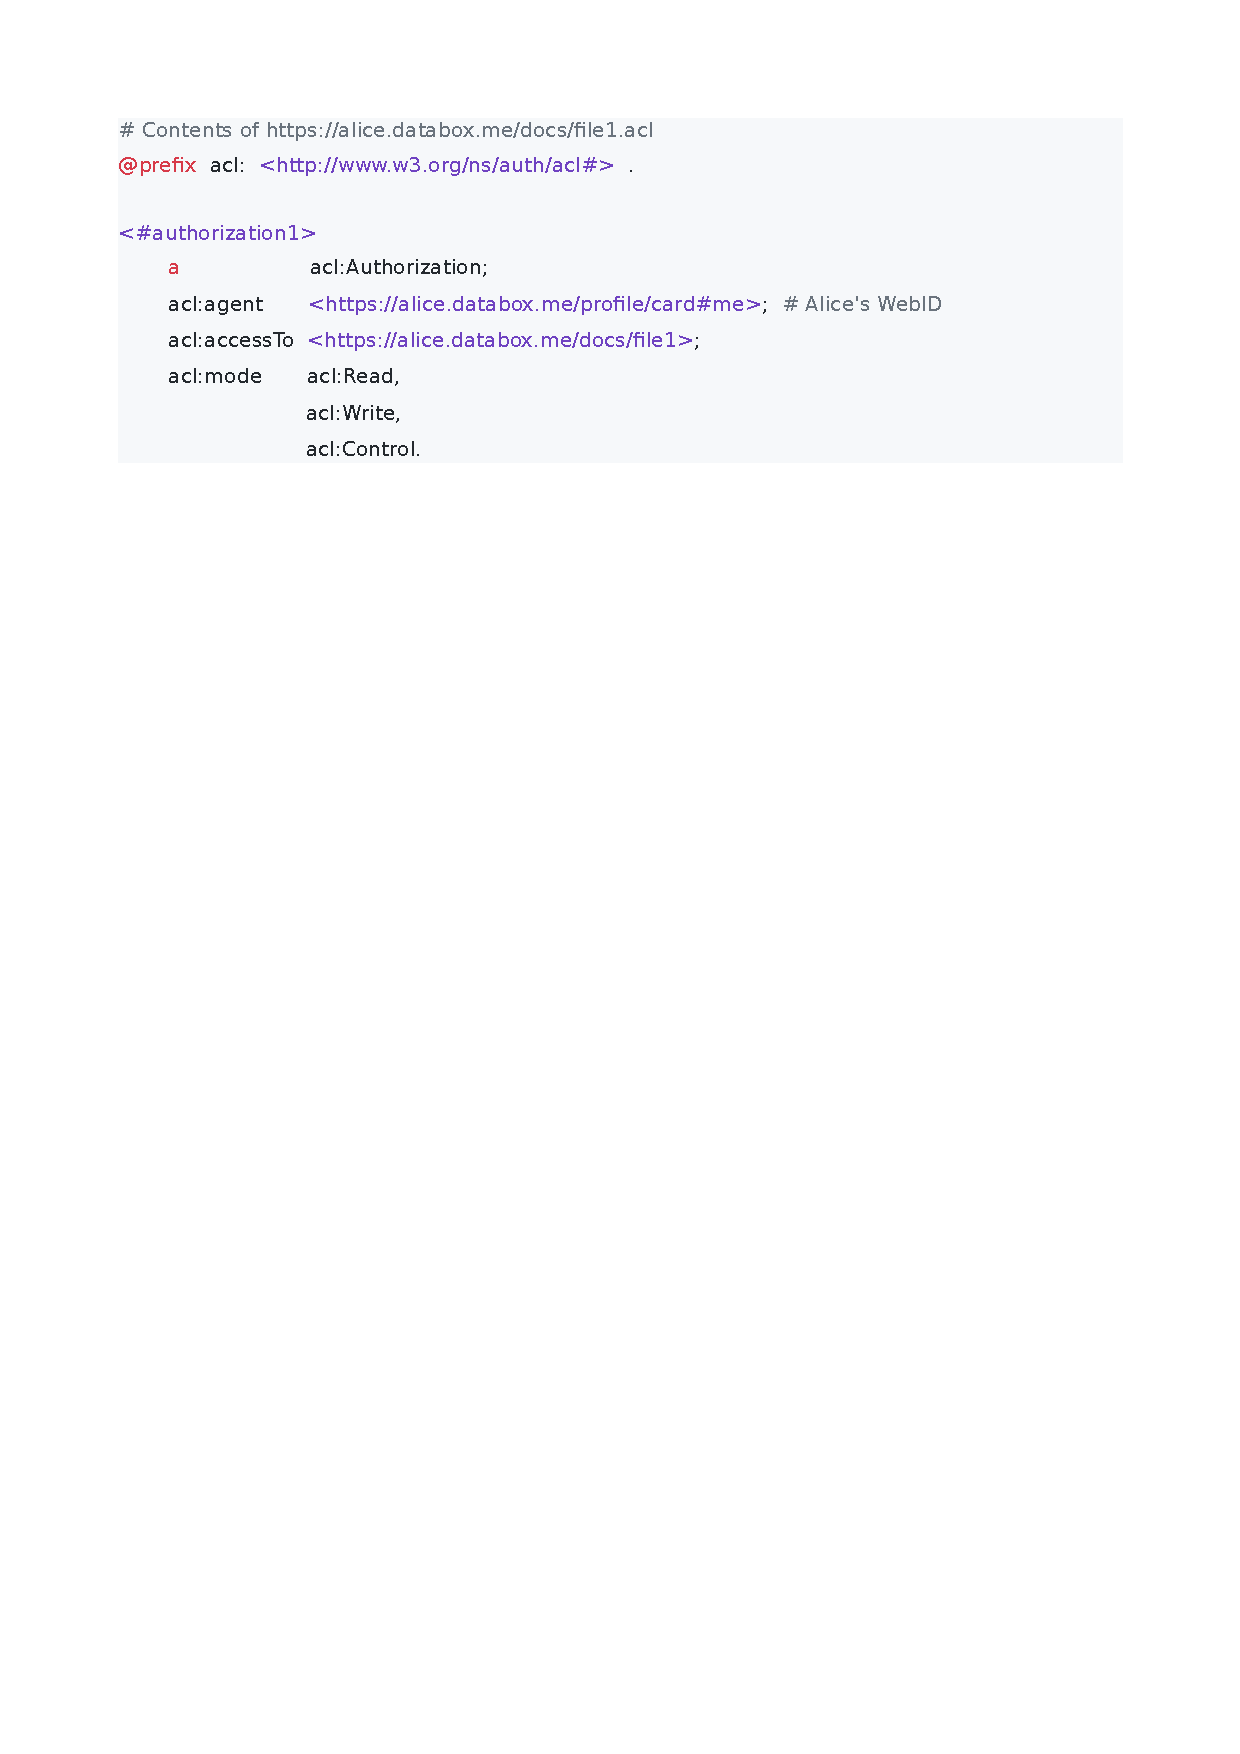
\includegraphics[trim=2cm 21.9cm 4.7cm 2cm, clip, scale=0.57]{pdf/alice-permission}|
\end{lstlisting}

Listing \ref{lst:individual-permission} shows an example of a WAC document that specifies that Alice (as identified by her WebID \code{https://alice.\\databox.me/profile/card\#me}) has full access (read, write, and control) to one of her web resources, located at \code{https://\\alice.databox.me/docs/file1}.

Similarly, it is possible to give access to a group of agents using the \code{acl:agentGroup} predicate. A group is a collection of members (or WebIDs) that needs to be specified in a different file. Moreover, it is possible to give access to all agents (public access) or yet to all authenticated agents. It is also possible to classify Web Apps as trusted. Furthermore, not every document needs its own individual access control list file. Rather, it is possible to create an authorization to a container, which is a web location that contain multiple resources.

%%%%%%%%%%%%%%%%%%%%%%%%%%%%%%%%%%%%%%%%%%%%%%
%%%%% NEW SECTION
%%%%%%%%%%%%%%%%%%%%%%%%%%%%%%%%%%%%%%%%%%%%%%
\section{Esfinge Guardian}

In this section, we present the Esfinge Guardian\footnote{\url{https://github.com/EsfingeFramework/guardian}} framework.

Essentially, the Esfinge Guardian's role is to intercept calls to protected operations. Figure \ref{fig:interception-mechanism} depicts the interception. As an example, consider a protected operation \verb|debit()|, which should only be executed by the account owner. The call to \verb|debit()| would be intercepted by Esfinge Guardian.

\begin{figure}
  \centering
  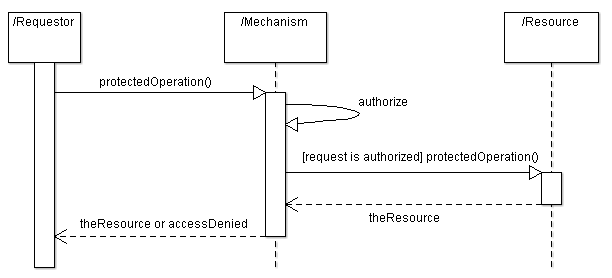
\includegraphics[scale=0.5]{img/interception-mechanism.png}
  \caption{A conceptualization of the interception mechanism (Silva et al. \cite{Silva2013})}
  \label{fig:interception-mechanism}
\end{figure}

Esfinge Guardian is composed of eight main elements (see Guerra et al. \cite{Guerra2015} and Silva et al.\cite{Silva2013} for in depth explanations). For brevity, we only present the three elements necessary to implement access control policies of our case example.

\noindent \verb|AuthorizationContext|. It is the central entity that holds all the information required for an authorization, which includes the data for the subject, resource, and environment. That means all other entities should provide AuthorizationContext with enough information for authorization to occur.

\noindent \verb|Authorizer|: Entity that implements the logic of the access control policy and may use information stored in AuthorizationContext if necessary. There must be at least one Authorizer. Every Authorizer must provide a response in the form of a "yes" or "no"; however, it must be possible to include other response types such as "Indeterminate."


\noindent \verb|AuthorizationMetada|: Entity that indicates which resources – or their operations – must be intercepted by the authorization mechanism. A requirement is that this element must be of metadata type so that it can be used declaratively. Esfinge Guardian uses Java annotations as the implementation of this element; however, it can be considered a general marking element that is independent of a specific technology.


%%%%%%%%%%%%%%%%%%%%%%%%%%%%%%%%%%%%%%%%%%%%%%
%%%%% NEW SECTION
%%%%%%%%%%%%%%%%%%%%%%%%%%%%%%%%%%%%%%%%%%%%%%
\section{Case Example}

In this section, we present how Esfinge Guardian provides developers with appropriate tools for separating business concerns from the authorization logic without compromising simplicity.

We expand the example previously presented in the introduction. Consider the following access control policy of a hypothetical bank Web App. \textit{Only managers can read sensitive data from the users' pods as long as they are inside the bank facilities}.

Esfinge Guardian requires three steps for implementing this access control policy. The first step is to implement authorizers, which contain the authorization logic, as shown in Listing \ref{lst:authorizers}. \verb|ManagerAuthorizer| is responsible for authorizing managers while \verb|WithinFacilitiesAuthorizer| authorizes based on the users' location.

\begin{lstlisting}[escapeinside=||,caption={Manager and WithinFacilities Authorizers}, captionpos=b,label={lst:authorizers}]
  |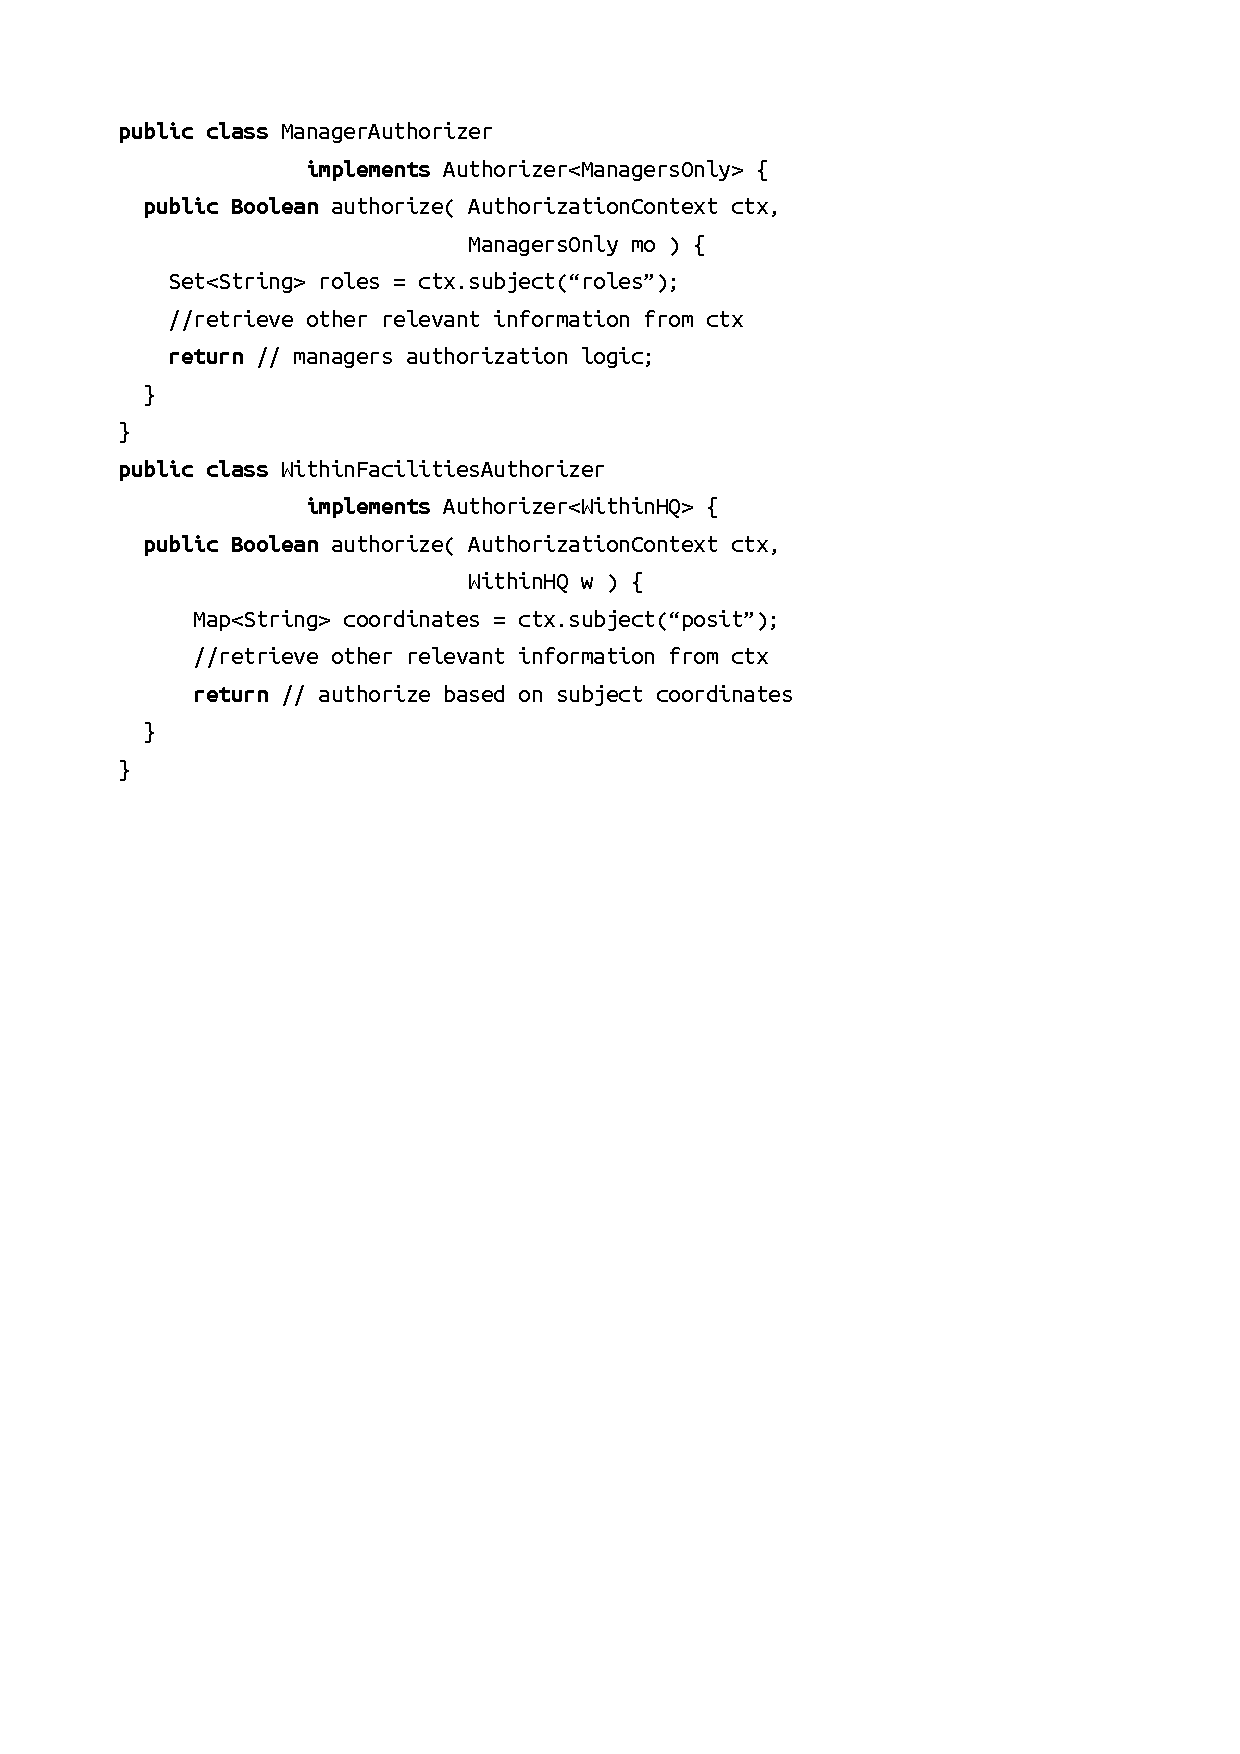
\includegraphics[trim=2cm 16.5cm 2.7cm 2.1cm, clip, scale=0.67]{pdf/authorizers}|
\end{lstlisting}

The second step requires the binding of authorizers to domain annotations, as shown in Listing \ref{lst:binding-annotations}.

\begin{lstlisting}[escapeinside=||,caption={Binding authorization annotations with respective implementations}, captionpos=b,label={lst:binding-annotations}]
  |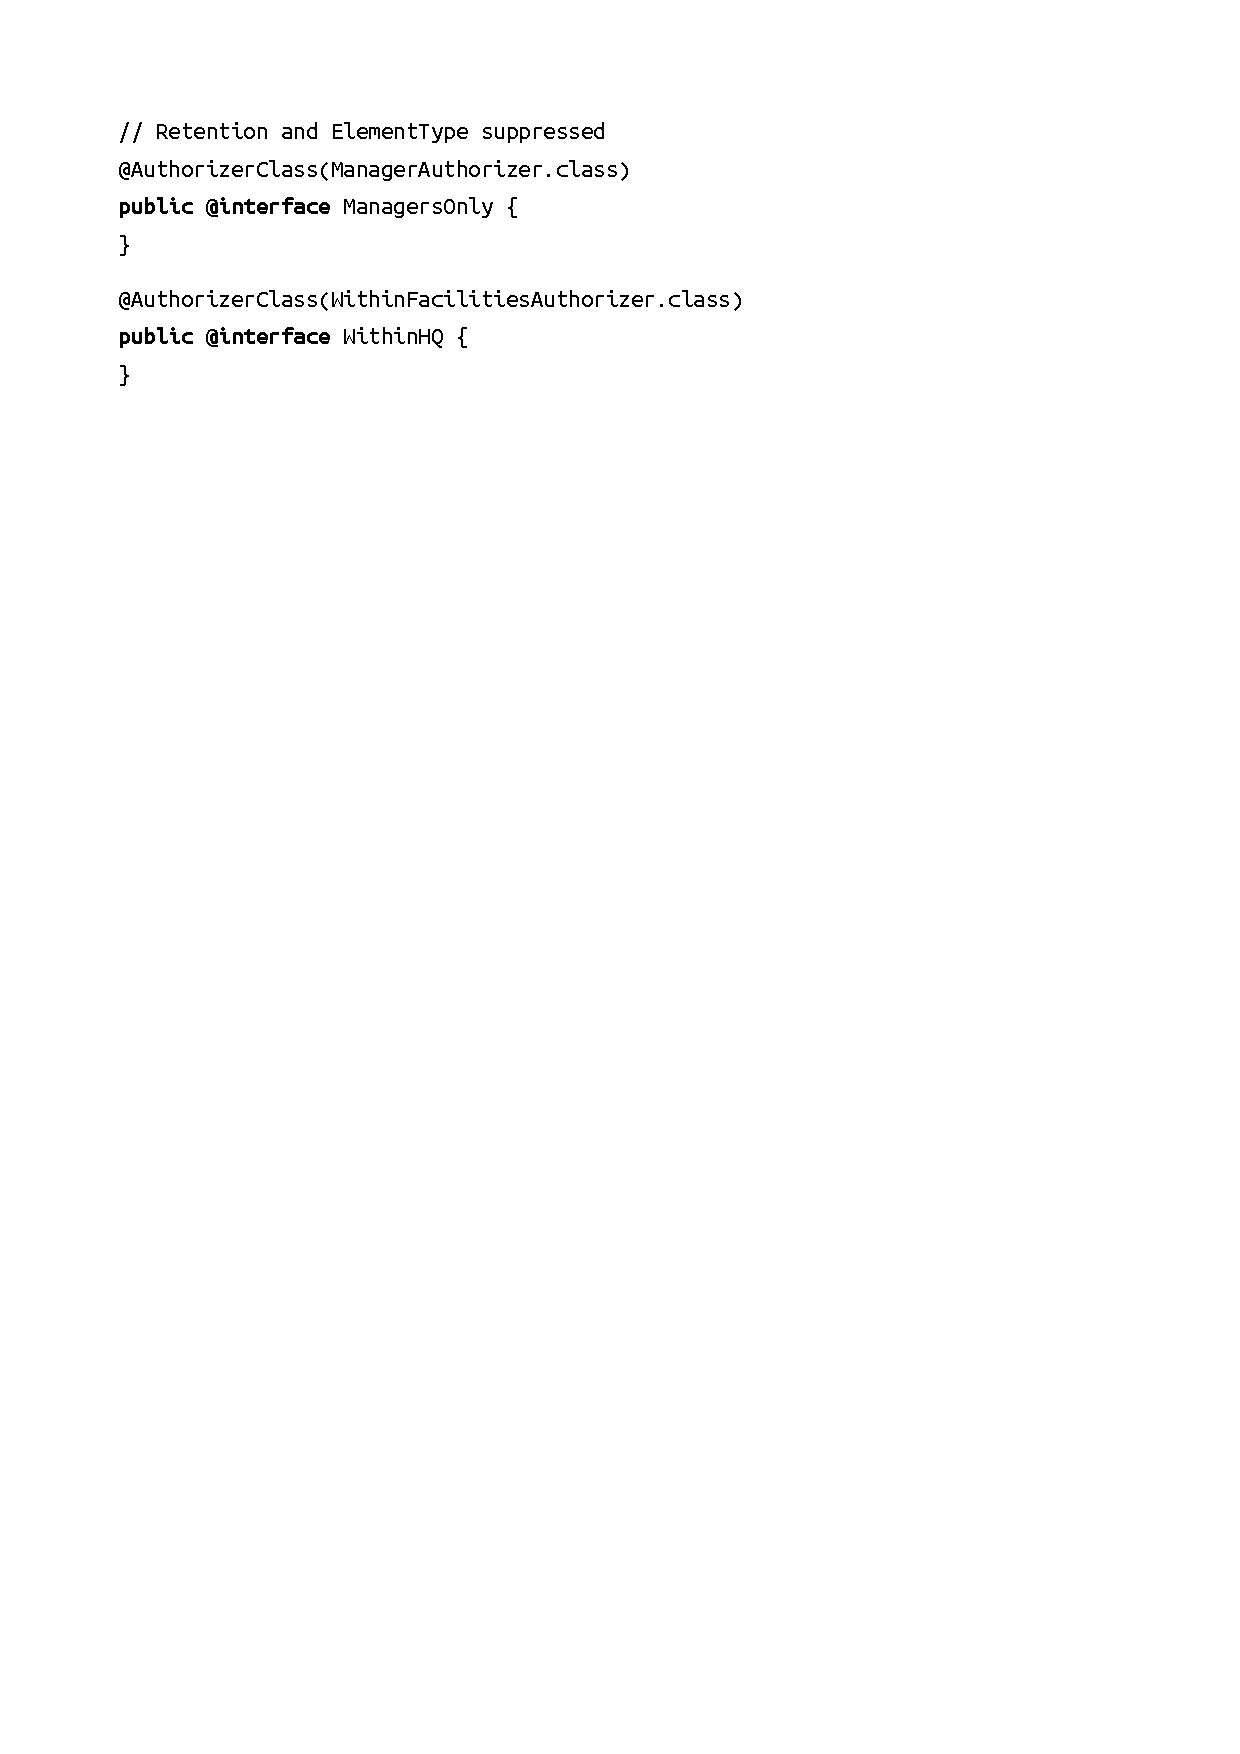
\includegraphics[trim=2cm 23.1cm 2.7cm 2.7cm, clip, scale=0.67]{pdf/binding-authorization-annotations}|
\end{lstlisting}

Finally, developers should use the domain annotations (\verb|@ManagersOnly| and \verb|@WithinHQ|) to protect sensitive operations, as presented in Listing \ref{lst:business-method}.

\begin{lstlisting}[escapeinside=||,caption={A Web App method that reads sensitive data from users with access control managed by Esfinge Guardian}, captionpos=b,label={lst:business-method}]
  |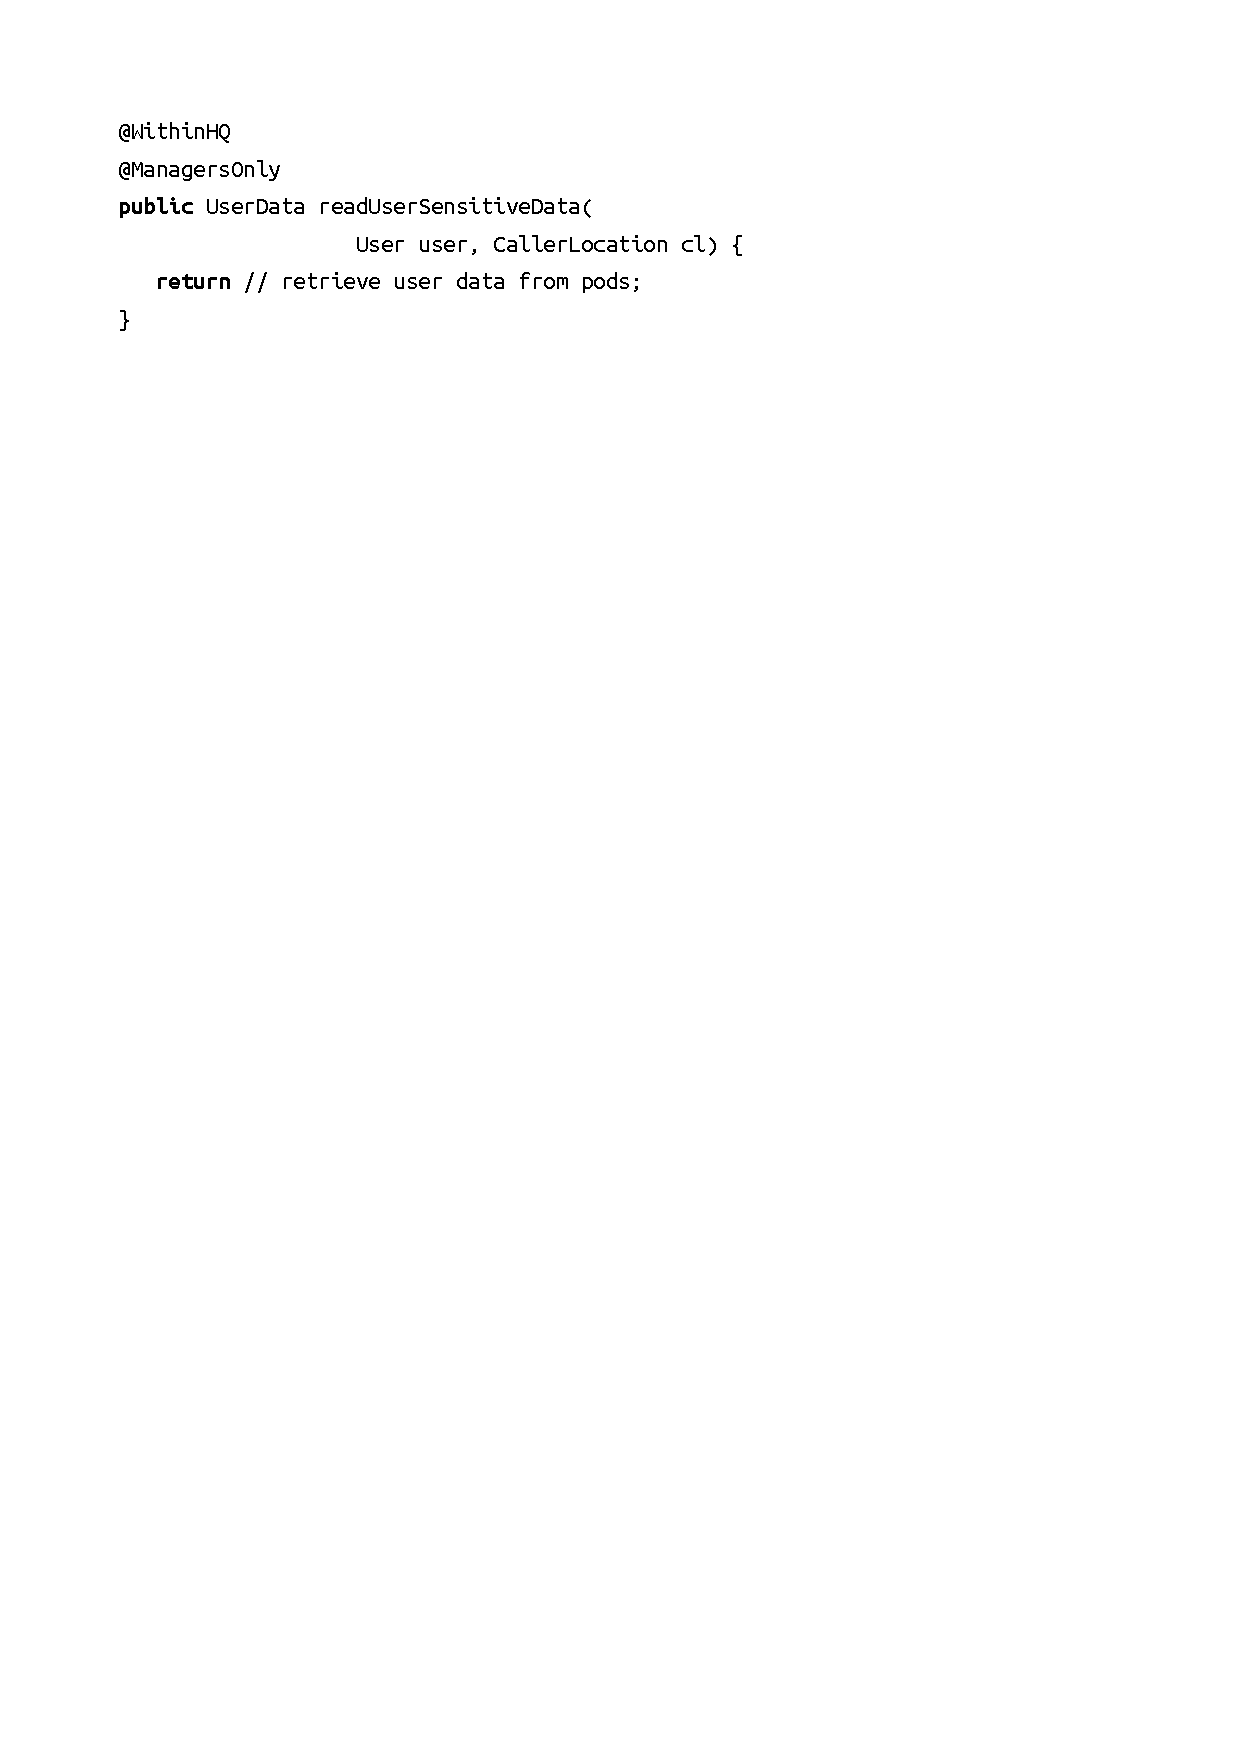
\includegraphics[trim=2cm 24cm 5cm 2.1cm, clip, scale=0.67]{pdf/business-method-impl}|
\end{lstlisting}

We list two benefits of using Esfinge Guardian for managing access control in decentralized Web Apps compliant to LGPD. First, by providing a mechanism for separating authorization from business concerns, Esfinge Guardian eases that a specialized privacy team to work independently from other software engineers (the principle of least privilege). In this way, only the developers in the privacy team would become liable in case of data breaches. Second, the use of domain annotations makes the code more readable for audits.


\section{Related Works}

The new regulations about data protection (i.e. GDPR, LGDP) bring new technical challenges related to how applications will handle personal data still be in compliance the law in terms of privacy. Application vendors are already able to guarantee compliance to these regulations in their tools in terms of consent management and personal data tracking, although data portability and interoperability among different products and services are still big challenges to tackle.

According to \cite{bonatti2018data}, it is necessary to have tools and best practices to help building privacy-by-design systems\cite{cavoukian2009privacy}. Authors argue that the standardization work in this domain still have to address the interoperability challenge. There are no standard ontology that align the terminology of privacy legislation with vocabularies to describe and interchange data, thus enabling personal data portability.

There are ongoing initiatives putting together efforts to develop vocabularies and standards to enable semantic interoperability and transparency logs about personal data processing. A primary forum working on this matter is the 'W3C Community Group' entitled \textit{Data Privacy Vocabularies and Controls CG}.

Performance is an issue in the decentralization model\cite{verborgh_iswc_2018}. The heterogeneity and distribution of a decentralized network implies that data processing algorithms will require more computational resources to perform tasks, comparing it with the centralized ones.

Author points out that federated SPARQL query engines perform better in private networks instead of on the public Web. Thus, a suitable alternative to overcome this issue is the promising \linebreak \textit{Linked Data Fragments}\cite{LDF}, less expressive query interfaces.

\section{Discussion and Conclusion}

The LGPD requires companies to adopt a comprehensive data governance approach, including data profiling, data lineage, data masking, test-data management, and data archives. Also, specialized professionals are required to design and handle personal data.

In this work, we show how Esfinge Guardian can be used to manage authorizations in decentralized Web Apps to increase compliance with the LGPD's data governance requirements. Besides the offered examples, Esfinge Guardian could be used to anonymize personal data, with the Authorizers filtering information that could lead to users identification.

%
% The acknowledgments section is defined using the "acks" environment (and NOT an unnumbered section). This ensures
% the proper identification of the section in the article metadata, and the consistent spelling of the heading.
\begin{acks}
To the Brazilian Network Information Center (NIC.br) and Web Technologies Study Center (Ceweb.br) for supporting this research.
\end{acks}

%
% The next two lines define the bibliography style to be used, and the bibliography file.
\bibliographystyle{ACM-Reference-Format}
\bibliography{laweb19}


\end{document}
